%========================================================================================
%   Clase 2: Analisis exploratorio y procesamiento de datos
%   Analitica de Datos - Maestria en Ciencias del Comportamiento (UdeSA)
%   Plantilla: SimpleDarkBlue con primario UdeSA (aprobada) + logo institucional
%========================================================================================
\documentclass[aspectratio=169,xcolor=dvipsnames]{beamer}
\usetheme{SimpleDarkBlue}
\useoutertheme[subsection=false]{miniframes}  % navegacion de circulos (uno por slide, por seccion)

\usepackage[utf8]{inputenc}
\usepackage[T1]{fontenc}
\usepackage[spanish,es-noshorthands]{babel}
\usepackage{graphicx}
\usepackage{booktabs}
\usepackage{listings}
\usepackage{tikz}

\usepackage[scaled]{helvet}
\renewcommand{\familydefault}{\sfdefault}

\graphicspath{{./}}

% --- Estilo de codigo Python (listings) ---
\lstdefinestyle{py}{%
    language=Python,
    basicstyle=\ttfamily\footnotesize,
    keywordstyle=\color{udesaNavy}\bfseries,
    commentstyle=\color{tabGray}\itshape,
    stringstyle=\color{tabGreen},
    showstringspaces=false,
    backgroundcolor=\color{blockBodyBg},
    frame=none,
    xleftmargin=0.6em, framexleftmargin=0.6em,
    breaklines=true, columns=fullflexible, keepspaces=true,
    aboveskip=0.5em, belowskip=0.3em,
}
\lstset{style=py}

% --- Primario UdeSA; secundarios = paleta del skill (tab20c) ---
\definecolor{udesaNavy}{HTML}{00529B}
\definecolor{tabBlue}{HTML}{3182BD}
\definecolor{tabOrange}{HTML}{E6550D}
\definecolor{tabOrangeLL}{HTML}{FDD0A2}
\definecolor{tabGreen}{HTML}{31A354}
\definecolor{tabGreenLL}{HTML}{C7E9C0}
\definecolor{tabPurple}{HTML}{756BB1}
\definecolor{tabGray}{HTML}{636363}
\definecolor{tabGrayL}{HTML}{969696}
\definecolor{blockBodyBg}{HTML}{ECECEC}

\setbeamercolor{structure}{fg=udesaNavy}
\setbeamercolor{title}{bg=udesaNavy,fg=white}
\setbeamercolor{frametitle}{bg=udesaNavy,fg=white}
\setbeamercolor{block title}{fg=white,bg=udesaNavy}
\setbeamercolor{block body}{fg=black,bg=blockBodyBg}
\setbeamercolor{block title example}{fg=white,bg=tabGreen}
\setbeamercolor{block body example}{fg=black,bg=tabGreenLL}
\setbeamercolor{block title alerted}{fg=white,bg=tabOrange}
\setbeamercolor{block body alerted}{fg=black,bg=tabOrangeLL}
\setbeamercolor{alerted text}{fg=tabOrange}
\setbeamercolor{itemize item}{fg=udesaNavy}
\setbeamercolor{itemize subitem}{fg=udesaNavy}
\setbeamercolor{enumerate item}{fg=udesaNavy}

% --- Tematizacion por bloque: la BARRA de titulo toma el color del bloque (separacion fuerte) ---
\newcommand{\bloque}[1]{%
    \setbeamercolor{frametitle}{bg=#1,fg=white}%
    \setbeamercolor{structure}{fg=#1}%
    \setbeamercolor{alerted text}{fg=#1}%
    \setbeamercolor{itemize item}{fg=#1}%
    \setbeamercolor{itemize subitem}{fg=#1}%
    \setbeamercolor{enumerate item}{fg=#1}%
}
% Apertura/cierre: barra navy (identidad institucional)
\newcommand{\navytheme}{\bloque{udesaNavy}}

% --- Logo UdeSA (blanco) arriba a la derecha en las slides de contenido ---
\setbeamertemplate{frametitle}{%
    \nointerlineskip
    \begin{beamercolorbox}[wd=\paperwidth,ht=2.7ex,dp=1.3ex,leftskip=0.4cm,rightskip=0.4cm]{frametitle}%
        \usebeamerfont{frametitle}\insertframetitle%
        \hfill\raisebox{-0.2ex}{
\includegraphics[height=2.1ex]{udesa-logo-color-white.png}}%
    \end{beamercolorbox}%
}

% --- Portada: logo a color (chico) arriba, luego el bloque de titulo ---
\titlegraphic{
\includegraphics[width=0.27\textwidth]{udesa-logo-color.png}}
\makeatletter
\setbeamertemplate{title page}{%
    \vspace{2.0em}
    \begingroup
    \centering
    {\inserttitlegraphic\par}
    \vskip2.0em
    \begin{beamercolorbox}[sep=10pt,center,shadow=true,rounded=true]{title}
        \usebeamerfont{title}\inserttitle\par%
        \ifx\insertsubtitle\@empty\else%
        \vskip0.4em{\large\usebeamercolor[fg]{subtitle}\insertsubtitle\par}%
        \fi%
    \end{beamercolorbox}%
    \vskip1.2em\par
    {\large\textbf{\insertauthor}\par}%
    \vskip0.25em
    {\small\insertdate\par}%
    \endgroup
    \vfill
}
\makeatother

% --- Navegacion: un circulo por slide, agrupados por bloque (seccion), en el footer ---
\AtBeginSection{}                  % que \section no genere una slide automatica
\setbeamertemplate{headline}{}     % sin barra de navegacion arriba (va en el footer)
% Base (otras secciones) = gris hueco/vacio; solo la seccion ACTUAL toma el color del bloque
\setbeamercolor{mini frame}{fg=gray!55, bg=white}
\setbeamercolor{mini frame in current subsection}{use=structure, fg=structure.fg, bg=structure.fg!30}
\setbeamercolor{mini frame in other subsection}{fg=gray!55, bg=white}
\setbeamercolor{section in head/foot}{fg=gray!60}
\setbeamercolor{subsection in head/foot}{fg=gray!60}
% El footer (nombres + circulos) recien aparece cuando arranca el primer bloque
\setbeamertemplate{footline}{%
    \ifnum\insertsectionnumber>0%
        \vskip2pt%
        \hbox to\paperwidth{%
            \hskip0.5cm%
            \raisebox{0.2ex}{\insertnavigation{\dimexpr\paperwidth-1cm\relax}}%
            \hss%
        }%
        \vskip3pt%
    \fi%
}

\title{Clase 2:\\ \textbf{An\'alisis exploratorio y procesamiento de datos}}
\subtitle{Anal\'itica de Datos}
\author{Maestr\'ia en Ciencias del Comportamiento}
\date{Primavera 2026}

\begin{document}

%======================= APERTURA =======================
\navytheme

% -- 1. Portada --
\begin{frame}[plain]\titlepage\end{frame}

% -- 2. Pregunta guia + preview del dataset --
\begin{frame}{}
    \vfill
    \begin{center}
        {\Large ?`Qui\'enes dejan una empresa, y \alert{por qu\'e}?}\\[0.7em]
        {\footnotesize Un caso real de \emph{people analytics}: rotaci\'on de personal (dataset HR Attrition, 1470 empleados).}\\[0.9em]
        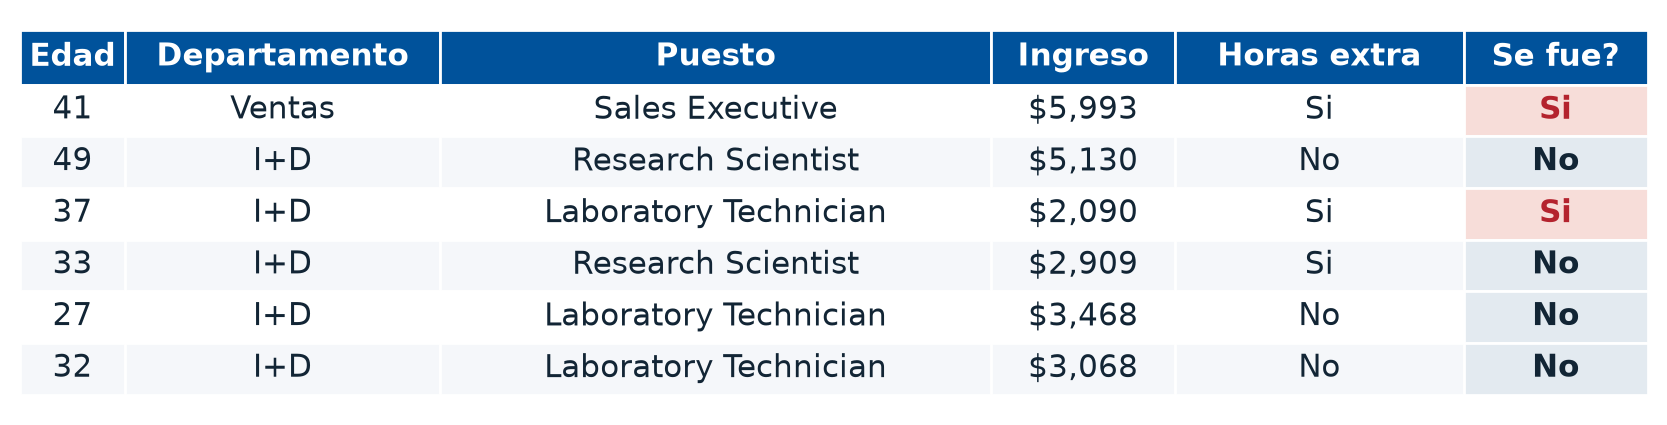
\includegraphics[width=0.95\linewidth]{clase02_dataset_preview.png}
    \end{center}
    \vfill
\end{frame}

% -- 3. Objetivo + roadmap --
\begin{frame}{De qu\'e vamos a hablar hoy}
    \begin{block}{Objetivo}
        Aprender los \textbf{fundamentos de Python} para el an\'alisis de datos y recorrer, de punta a punta, el \textbf{an\'alisis exploratorio (EDA)} sobre datos reales.
    \end{block}
    \begin{enumerate}
        \item \textbf{Fundamentos de Python y carga de datos.} Variables, estructuras y funciones; del archivo al DataFrame.
        \item \textbf{Explorar.} Tipos, estructura y estad\'isticos descriptivos.
        \item \textbf{Procesar y limpiar.} Filtrar y agrupar; tratar faltantes, duplicados y outliers.
        \item \textbf{Transformar.} Crear variables con sentido (\emph{feature engineering}) y fijar el vocabulario.
    \end{enumerate}
    \vfill
    \begin{center}
        {\normalsize Para las pr\'acticas vamos a ir a~\href{https://colab.research.google.com/github/tomdamelio/analitica_de_datos/blob/main/clases/clase-02/notebooks/clase02_python.ipynb}{\raisebox{-0.32\height}{
\includegraphics[height=3.4ex]{colab_logo.png}}~\textbf{Colab}}.}
    \end{center}
\end{frame}

%======================= BLOQUE 1: Fundamentos de Python + carga =======================
\section{Fundamentos de Python y carga}
\bloque{tabBlue}

% -- Divisor --
\begin{frame}{}
    \vfill
    \begin{center}
        {\small\textbf{\color{tabBlue}BLOQUE 1 DE 4}}\\[0.5em]
        {\Large\textbf{Fundamentos de Python y carga de datos}}\\[0.8em]
        {\normalsize Del lenguaje a la primera tabla de datos.}
    \end{center}
    \vfill
\end{frame}

% -- Python con R al lado --
\begin{frame}{Python, con R al lado}
    Nos apoyamos en lo que ya saben: cada operaci\'on tiene su equivalente en R.
    \vskip0.6em
    \begin{center}
    {\footnotesize
    \begin{tabular}{@{}lll@{}}
        \toprule
        \textbf{en R (tidyverse)} & \textbf{en Python (pandas)} & \textbf{qu\'e hace} \\
        \midrule
        \texttt{x <- 42} & \texttt{x = 42} & asignar una variable \\
        \texttt{c(29, 41, 35)} & \texttt{[29, 41, 35]} & colecci\'on ordenada \\
        \texttt{list(a = 1)} & \texttt{\{"a": 1\}} & colecci\'on con nombres \\
        \texttt{for (x in xs) \{ \}} & \texttt{for x in xs:} & recorrer \\
        \texttt{if (c) \{ \} else \{ \}} & \texttt{if c: ... else:} & condicional \\
        \texttt{f <- function(x) \{ \}} & \texttt{def f(x):} & definir una funci\'on \\
        \bottomrule
    \end{tabular}}
    \end{center}
    \vfill
    {\footnotesize \alert{Ojo:} en Python la \textbf{indentaci\'on} (no las llaves) define los bloques, y se cuenta \textbf{desde 0}.}
\end{frame}

% -- Variables, tipos, estructuras --
\begin{frame}[fragile]{Variables, tipos y estructuras}
\begin{lstlisting}
edad = 34                # int   (entero)
ingreso = 4919.0         # float (decimal)
puesto = "Sales Exec"    # str   (texto)
renuncio = False         # bool  (True / False)

# una lista de diccionarios ya ES una tabla en miniatura
equipo = [{"nombre": "Ana",   "renuncio": True},
          {"nombre": "Bruno", "renuncio": False}]
\end{lstlisting}
    \begin{itemize}
        \item El \textbf{tipo} determina qu\'e pod\'es hacer con el valor.
        \item \textbf{Lista}: valores en orden (el primero es el \texttt{[0]}). \textbf{Diccionario}: pares \emph{nombre: valor}, una observaci\'on.
    \end{itemize}
\end{frame}

% -- Control de flujo y funciones --
\begin{frame}[fragile]{Control de flujo y funciones}
\begin{lstlisting}
def tasa_de_renuncia(personas):
    renuncias = 0
    for p in personas:          # recorrer la coleccion
        if p["renuncio"]:       # decidir segun una condicion
            renuncias += 1
    return renuncias / len(personas)
\end{lstlisting}
    \begin{itemize}
        \item \texttt{for} recorre, \texttt{if} decide, \texttt{def} empaqueta un c\'alculo para \textbf{reutilizarlo}.
        \item Idea que usaremos todo el tiempo: la \textbf{media de una columna de True/False es una proporci\'on}.
    \end{itemize}
\end{frame}

% -- Del archivo al DataFrame --
\begin{frame}[fragile]{Del archivo al DataFrame}
\begin{lstlisting}
import pandas as pd
url = "https://.../emp_attrition.csv"
df = pd.read_csv(url)     # tambien read_excel(...), read_parquet(...)
df.shape                  # (1470, 35): filas x columnas
\end{lstlisting}
    \begin{itemize}
        \item Un \textbf{DataFrame} es una tabla: cada \textbf{fila} una observaci\'on, cada \textbf{columna} una variable.
        \item Cargamos desde una \textbf{URL} p\'ublica para que funcione en Colab sin archivos locales.
    \end{itemize}
\end{frame}

% -- Importar y exportar formatos --
\begin{frame}[fragile]{Importar y exportar: CSV, Excel, parquet}
\begin{lstlisting}
df = pd.read_csv(url)             # tambien read_excel(...), read_parquet(...)
df.to_csv("hr.csv", index=False)  # guardar: to_excel(...), to_parquet(...)
\end{lstlisting}
    \begin{itemize}
        \item Por cada \texttt{read\_*} hay un \texttt{to\_*}: cargar y guardar son \textbf{sim\'etricas}.
        \item \textbf{CSV} (universal), \textbf{Excel} (planillas), \textbf{parquet} (columnar: r\'apido y liviano para datos grandes).
        \item \texttt{read\_csv} tiene par\'ametros para archivos sucios: \texttt{sep}, \texttt{na\_values}, \texttt{usecols}, \texttt{encoding}.
    \end{itemize}
\end{frame}

% -- A la notebook (Ejercicio 1) --
\begin{frame}{}
    \vfill
    \begin{center}
        \href{https://colab.research.google.com/github/tomdamelio/analitica_de_datos/blob/main/clases/clase-02/notebooks/clase02_python.ipynb}{
\includegraphics[height=7ex]{colab_logo.png}}\\[0.6em]
        {\Large\textbf{A la notebook}}\\[0.6em]
        {\normalsize \textbf{Ejercicio 1:} clasificar ingresos con una funci\'on y un \texttt{for}.}\\[0.4em]
        {\footnotesize Practicamos los fundamentos y cargamos el dataset, en Python o en R.}
    \end{center}
    \vfill
\end{frame}

%======================= BLOQUE 2: Explorar (tipos, estructura, descriptivos) =======================
\section{Explorar}
\bloque{tabOrange}

% -- Divisor --
\begin{frame}{}
    \vfill
    \begin{center}
        {\small\textbf{\color{tabOrange}BLOQUE 2 DE 4}}\\[0.5em]
        {\Large\textbf{Explorar: tipos, estructura y descriptivos}}\\[0.8em]
        {\normalsize Antes de modelar, mirar; antes de mirar, resumir.}
    \end{center}
    \vfill
\end{frame}

% -- Primer vistazo --
\begin{frame}[fragile]{Primer vistazo al dataset}
\begin{lstlisting}
df.shape          # (1470, 35): 1470 empleados, 35 variables
df.info()         # tipo y no-nulos de cada columna
df["Attrition"].value_counts()    # No: 1233 | Yes: 237
\end{lstlisting}
    \begin{itemize}
        \item Leer los \textbf{tipos} es el primer chequeo de calidad: 26 columnas num\'ericas y 9 de texto.
        \item Una variable num\'erica que aparece como \emph{texto} es se\~nal de \textbf{datos sucios}.
    \end{itemize}
\end{frame}

% -- Distribucion del ingreso (figura) --
\begin{frame}{La mitad gana menos de \$4.919: la media la infla la cola}
    \centering
    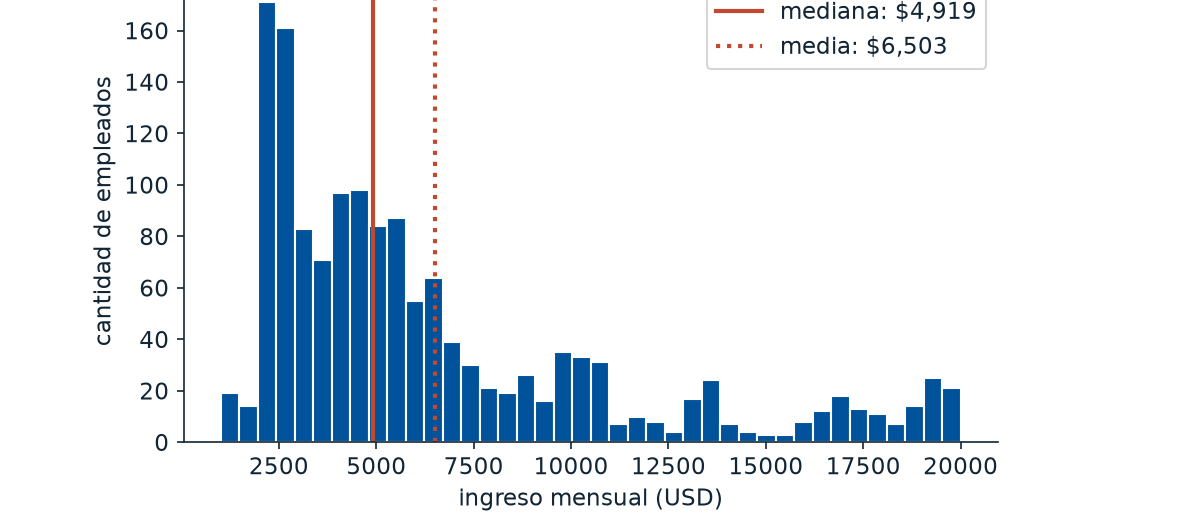
\includegraphics[width=\linewidth,height=0.74\textheight,keepaspectratio]{clase02_distribucion_ingreso_notitle.png}\\
    {\footnotesize Distribuci\'on del ingreso mensual (n = 1470). \textbf{Mediana \$4.919} frente a \textbf{media \$6.503}: la cola de sueldos altos empuja la media.}
\end{frame}

% -- La trampa: media vs mediana --
\begin{frame}{La trampa: media frente a mediana}
    \begin{alertblock}{Cuidado}
        Cuando la distribuci\'on es \textbf{asim\'etrica}, la \textbf{media} deja de describir al caso ``t\'ipico''.
    \end{alertblock}
    \begin{itemize}
        \item Los ingresos tienen \textbf{asimetr\'ia a derecha}: unos pocos sueldos altos \alert{empujan la media hacia arriba}.
        \item Para el ingreso ``t\'ipico'' se reporta la \textbf{mediana} (\$4.919), no la media (\$6.503).
        \item Regla general: \textbf{mir\'a la distribuci\'on}, no solo un promedio.
    \end{itemize}
\end{frame}

%======================= BLOQUE 3: Procesar y limpiar con pandas =======================
\section{Procesar y limpiar}
\bloque{tabGreen}

% -- Divisor --
\begin{frame}{}
    \vfill
    \begin{center}
        {\small\textbf{\color{tabGreen}BLOQUE 3 DE 4}}\\[0.5em]
        {\Large\textbf{Procesar y limpiar con pandas}}\\[0.8em]
        {\normalsize Filtrar, agrupar, y dejar los datos listos para modelar.}
    \end{center}
    \vfill
\end{frame}

% -- Verbos de pandas (mapa) --
\begin{frame}{Los verbos de todos los d\'ias}
    El 80\% del trabajo real son cuatro verbos que ya usaron en \texttt{dplyr}.
    \vskip0.5em
    \begin{center}
    {\footnotesize
    \resizebox{\textwidth}{!}{%
    \begin{tabular}{@{}lll@{}}
        \toprule
        \textbf{verbo} & \textbf{en dplyr (R)} & \textbf{en pandas} \\
        \midrule
        elegir columnas & \texttt{select(df, a, b)} & \texttt{df[["a", "b"]]} \\
        filtrar filas & \texttt{filter(df, cond)} & \texttt{df[cond]} \\
        ordenar & \texttt{arrange(df, desc(a))} & \texttt{df.sort\_values("a", ascending=False)} \\
        renombrar & \texttt{rename(df, n = viejo)} & \texttt{df.rename(columns=\{"viejo": "n"\})} \\
        agrupar y resumir & \texttt{group\_by() + summarise()} & \texttt{df.groupby("g")["x"].median()} \\
        \bottomrule
    \end{tabular}}}
    \end{center}
    \vfill
    {\footnotesize El filtro es una \textbf{m\'ascara booleana}: \texttt{df["OverTime"] == "Yes"} da una columna de True/False, y \texttt{df[mascara]} se queda con las filas True.}
\end{frame}

% -- Seleccionar con loc / iloc --
\begin{frame}[fragile]{Seleccionar con \texttt{loc} e \texttt{iloc}}
\begin{lstlisting}
df.loc[df["OverTime"]=="Yes", ["JobRole","MonthlyIncome"]]  # por etiqueta
df.iloc[:5, :3]                                             # por posicion (desde 0)
df["Age"]                                                   # es una Series
\end{lstlisting}
    \begin{itemize}
        \item \texttt{loc}: por \textbf{etiqueta} (nombres, \'indice). \texttt{iloc}: por \textbf{posici\'on} entera (desde 0).
        \item Una sola columna es una \textbf{Series} (un vector 1D con \'indice), el bloque con el que se arma el DataFrame.
    \end{itemize}
\end{frame}

% -- Limpieza estructural --
\begin{frame}[fragile]{Limpieza estructural}
\begin{lstlisting}
# columnas que valen lo mismo en las 1470 filas: no aportan
constantes = [c for c in df.columns if df[c].nunique() == 1]
df = df.drop(columns=constantes)  # EmployeeCount, Over18, StandardHours
df.duplicated().sum()             # 0 (en datos reales suelen aparecer)
\end{lstlisting}
    \begin{itemize}
        \item Una columna \textbf{constante} no distingue a nadie: fuera.
        \item \textbf{Duplicados} exactos: \texttt{duplicated()} para detectarlos, \texttt{drop\_duplicates()} para sacarlos.
    \end{itemize}
\end{frame}

% -- Faltantes: detectar -> decidir (figura) --
\begin{frame}{Faltantes: primero detectar, despu\'es decidir}
    \centering
    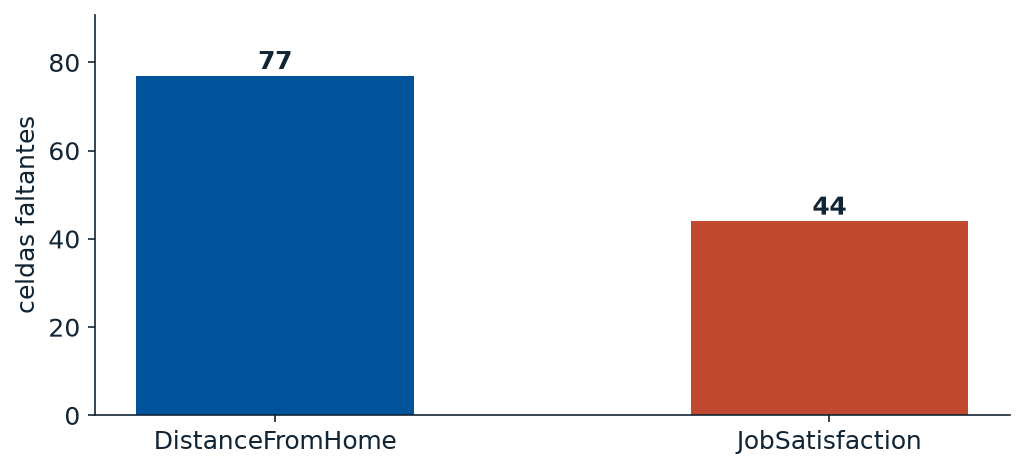
\includegraphics[width=0.72\linewidth,height=0.46\textheight,keepaspectratio]{clase02_faltantes_por_variable.png}
    \vskip0.3em
    \begin{itemize}
        \item \textbf{Eliminar} (\texttt{dropna}): simple, pero tira informaci\'on.
        \item \textbf{Imputar} (\texttt{fillna}): rellenar con un valor razonable (mediana para num\'ericas, moda para categor\'icas).
    \end{itemize}
    {\footnotesize Faltantes introducidos a prop\'osito para practicar (el dataset viene completo). La decisi\'on depende de \alert{cu\'anto} y \alert{por qu\'e} falta.}
\end{frame}

% -- Outliers (figura boxplot) --
\begin{frame}{Los 114 ingresos at\'ipicos: gerentes, no errores}
    \centering
    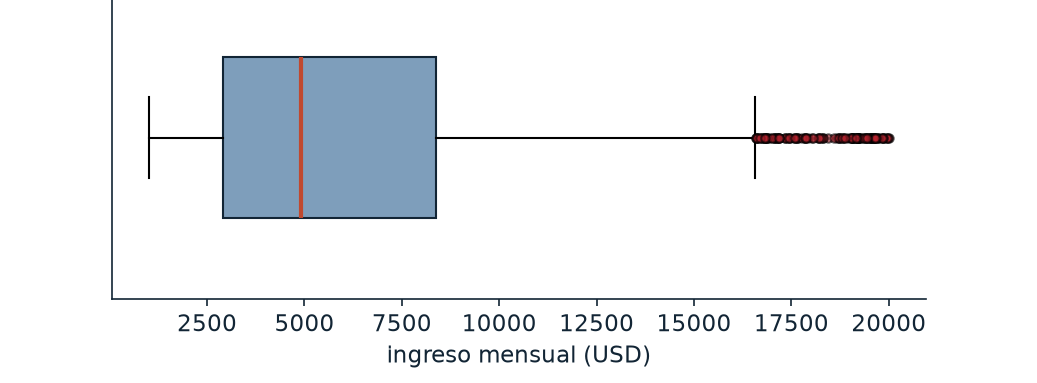
\includegraphics[width=\linewidth,height=0.66\textheight,keepaspectratio]{clase02_outliers_ingreso_notitle.png}\\
    {\footnotesize Regla del IQR: at\'ipico si supera $Q_3 + 1{,}5 \times IQR$. Los 114 puntos rojos son de nivel jer\'arquico 4 y 5: \textbf{at\'ipico no es sin\'onimo de error}.}
\end{frame}

% -- A la notebook (Ejercicios 2 y 3) --
\begin{frame}{}
    \vfill
    \begin{center}
        \href{https://colab.research.google.com/github/tomdamelio/analitica_de_datos/blob/main/clases/clase-02/notebooks/clase02_python.ipynb}{
\includegraphics[height=7ex]{colab_logo.png}}\\[0.6em]
        {\Large\textbf{A la notebook}}\\[0.6em]
        {\normalsize \textbf{Ejercicios 2 y 3:} tasa de rotaci\'on por puesto, e imputaci\'on por grupo.}\\[0.4em]
        {\footnotesize Procesar con pandas y tratar faltantes, en Python o en R.}
    \end{center}
    \vfill
\end{frame}

%======================= BLOQUE 4: Transformar =======================
\section{Transformar}
\bloque{tabPurple}

% -- Divisor --
\begin{frame}{}
    \vfill
    \begin{center}
        {\small\textbf{\color{tabPurple}BLOQUE 4 DE 4}}\\[0.5em]
        {\Large\textbf{Transformar: crear variables y nombrar}}\\[0.8em]
        {\normalsize Del dato limpio a variables con sentido para el an\'alisis.}
    \end{center}
    \vfill
\end{frame}

% -- Agrupar para comparar (figura attrition) --
\begin{frame}{Con horas extra, la rotaci\'on casi se \textbf{triplica}}
    \centering
    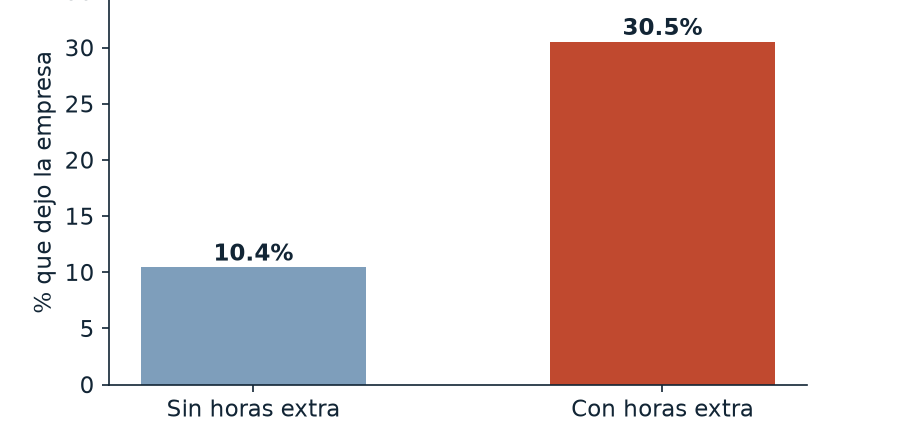
\includegraphics[width=\linewidth,height=0.70\textheight,keepaspectratio]{fig_attrition_extra.png}\\
    {\footnotesize Tasa de attrition seg\'un horas extra: \textbf{10,4\%} sin, \textbf{30,5\%} con (n = 1470). Un \texttt{groupby} + la media de una columna booleana responde cualquier ``tasa por grupo''.}
\end{frame}

% -- Feature engineering --
\begin{frame}[fragile]{Feature engineering: crear variables con sentido}
\begin{lstlisting}
# ingreso por anio de experiencia (dos trayectorias, mismo sueldo)
df["IngresoPorAnioExp"] = df["MonthlyIncome"] / (df["TotalWorkingYears"] + 1)

# discretizar la edad en tramos con etiqueta
df["TramoEdad"] = pd.cut(df["Age"], bins=[17, 30, 40, 50, 61],
                         labels=["18-30", "31-40", "41-50", "51-60"])
\end{lstlisting}
    \begin{itemize}
        \item Cuando ninguna columna captura el fen\'omeno, se \textbf{crea} una nueva.
        \item La justificaci\'on es el \alert{contexto} (el dominio), no el algoritmo.
    \end{itemize}
\end{frame}

% -- Terminologia (glosario) --
\begin{frame}{Un vocabulario com\'un}
    \begin{center}
    {\footnotesize
    \begin{tabular}{@{}ll@{}}
        \toprule
        \textbf{t\'ermino} & \textbf{qu\'e es} \\
        \midrule
        datos crudos & la fuente original, intacta \\
        limpieza & corregir errores, duplicados, tipos \\
        procesamiento & manipular: filtrar, agrupar, resumir \\
        preprocesamiento & lo que pide el algoritmo (estandarizar, imputar) \\
        \alert{feature engineering} & crear variables con sentido sustantivo \\
        feature selection & elegir qu\'e variables entran al modelo \\
        \bottomrule
    \end{tabular}}
    \end{center}
    \vfill
    {\footnotesize No es pedanter\'ia: en la Clase 4, confundir \emph{preprocesamiento} con \emph{procesamiento} puede invalidar un modelo (\textit{data leakage}).}
\end{frame}

% -- A la notebook (Ejercicio 4) --
\begin{frame}{}
    \vfill
    \begin{center}
        \href{https://colab.research.google.com/github/tomdamelio/analitica_de_datos/blob/main/clases/clase-02/notebooks/clase02_python.ipynb}{
\includegraphics[height=7ex]{colab_logo.png}}\\[0.6em]
        {\Large\textbf{A la notebook}}\\[0.6em]
        {\normalsize \textbf{Ejercicio 4:} el costo de viajar seguido (\emph{feature engineering}).}\\[0.4em]
        {\footnotesize Crear variables con sentido, en Python o en R.}
    \end{center}
    \vfill
\end{frame}

%======================= CIERRE =======================
\section{Cierre}
\navytheme

% -- Recap + hallazgo --
\begin{frame}{Lo que nos llevamos}
    \begin{block}{Ya pod\'es hacer un EDA de punta a punta}
        Cargar datos desde la nube, explorarlos, limpiarlos (faltantes, duplicados, outliers) y transformarlos (\emph{feature engineering}), en Python o en R.
    \end{block}
    \textbf{El hallazgo de hoy, en una frase:} en esta empresa la rotaci\'on se concentra en quienes
    \begin{itemize}
        \item hacen \textbf{horas extra} (30,5\% frente a 10,4\%),
        \item \textbf{viajan seguido} (24,9\%),
        \item y trabajan en \textbf{ventas} (39,8\% entre representantes).
    \end{itemize}
    \vfill
    {\footnotesize En la Clase 4 vamos a intentar \textbf{predecir} esa rotaci\'on.}
\end{frame}

% -- Lo que viene --
\begin{frame}{Lo que viene}
    \begin{itemize}
        \item \textbf{Clase 3:} visualizaci\'on de datos y reportes reproducibles (sobre este mismo dataset).
        \item \textbf{Lectura:} McKinney, \emph{Python for Data Analysis}, caps.\ 5 a 7 (gratis online).
        \item \textbf{Practicar:} las dos notebooks de hoy (Python y R) est\'an en el sitio de la materia.
    \end{itemize}
    \vfill
    \begin{center}
        {\Large\textbf{?`Preguntas?}}
    \end{center}
    \vfill
\end{frame}

\end{document}
